\documentclass[aspectratio=169,xcolor=dvipsnames]{beamer}
\usepackage{hyperref}
\usepackage{graphicx, animate}
\usepackage{booktabs}
\usepackage{bbm} % indicatrices

\usetheme{SimpleDarkBlue}

\newcommand{\bdOne}{\mathbbm{1}}

\title{Stratification: Monte Carlo and Simulation}
\author{
    Alban \textsc{Géron}, \\
    Arnaud \textsc{Barrat}, \\
    Camille \textsc{Legrée-Hagbarth}, \\
    Tristan \textsc{Fabre}
}
\date{April 29\textsuperscript{th}, 2025}



\begin{document}
    \begin{frame}
        \titlepage
    \end{frame}

    \begin{frame}{Introduction}
        We will study the integral of a periodic function which depends on the average of the input variables; more precisely, we have
        %
        \[f(u_1, \dots, u_d) = \varphi\left(\frac{u_1 + \cdots + u_d}{d}\right) \qquad \text{where } \varphi : \mathbb R \to \mathbb R \text{ is periodic}\]

        Such integrals exist in various applications: 
        \begin{itemize}
            \item \textbf{Physics:} modeling collective behavior in oscillatory systems or wave-based phenomena.
            \item \textbf{Machine Learning:} using periodic kernels in Gaussian Processes or kernel methods to model cyclical patterns.
            \item \textbf{Finance:} modeling seasonality or cyclic risk premiums based on averaged economic indicators.
            \item \textbf{Numerical Analysis:} benchmark function for evaluating Monte Carlo and variance reduction methods.
        \end{itemize}
        
    \end{frame}

    \begin{frame}{Problem}
        \begin{itemize}
            \item<1-> We seek to estimate the integral
            %
            \[I = \int_{[0, 1]^d} f(u) du \qquad \text{where } f(u_1, \dots, u_d) = \cos\left(2 \pi \left(\frac{1}{d} \sum_{i = 1}^d u_i - \frac{1}{2}\right)\right)\]

            \item<2-> For $d = 1$: $I = \int_0^1 \cos\left(2 \pi \left(u - \frac{1}{2}\right)\right) du = \frac{1}{2\pi} \int_{-\pi}^\pi \cos(t) dt = 0$.

            \item<3-> For large values of $d$: we have
            %
            \begin{align*}
                I &= \int_{[0, 1]^d} \varphi\left(\frac{u_1 + \cdots + u_d}{d}\right) du_1 \cdots du_d && \text{where } \varphi(t) = \cos\left(2 \pi \left(t - \frac{1}{2}\right)\right) \\
                &= \mathbb{E}\left[\varphi\left(\frac{U_1 + \cdots + U_d}{d}\right)\right] && \text{where } U_1, \dots, U_d \overset{\text{i.i.d.}}{\sim} \mathcal{U}([0, 1])
            \end{align*}
            %
            which converges to $\varphi(\mathbb{E}[U_1]) = 1$ by the law of large numbers, the continuous mapping theorem ($\varphi$ continuous) and the dominated convergence theorem ($\varphi$ bounded).
        \end{itemize}
    \end{frame}

    \begin{frame}{Summary}
        \tableofcontents
    \end{frame}

    \section{Estimation methods used to solve the problem (Monte-Carlo, quasi-Monte-Carlo)}

    \begin{frame}{Monte-Carlo}
        \begin{itemize}
            \item<1-> Notice that $I = \mathbb{E}[f(U)]$, where $U \sim \mathcal{U}([0, 1]^d)$.

            \item<2-> Thus, following Monte-Carlo's method, we approximate such an expectation by
            %
            \[\frac{1}{N} \sum_{n = 1}^N f(U_n)\]
            %
            where $N$ is a large integer and the $U_n$'s are $N$ i.i.d. random vectors uniformly distributed on $[0, 1]^d$.
        \end{itemize}
    \end{frame}

    \begin{frame}{Quasi-Monte-Carlo}
        \begin{itemize}
            \item<1-> In the course's slides, quasi-Monte-Carlo has been proven to be more efficient in terms of computation than Monte-Carlo, under weak assumptions.

            \item<2-> Again, we approximate $I = \mathbb{E}[f(U)]$ by an empirical mean of the form $\frac{1}{N} \sum_{n = 1}^N f(U_n)$. However here the $U_n$'s are generated in the set $\mathfrak{C}_N = \left\{\frac{1}{2N}, \frac{3}{2N}, \dots, \frac{2N - 1}{2N}\right\}^d$ under the condition \eqref{eq:cdC}:
            %
            \begin{equation}
                \alert{\text{each one of the points } U_1, \dots, U_N \text{ falls on exactly one strip of the set } \mathfrak{C}_N} \tag{C}\label{eq:cdC}
            \end{equation}

            \item<3-> For $d = 2$: the condition \eqref{eq:cdC} means that there is exactly one point in each line and each column:
            %
            \begin{center}
                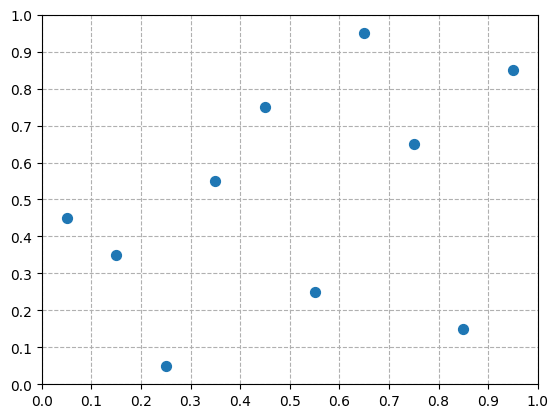
\includegraphics[width=0.3\textwidth]{points2.png}
            \end{center}
        \end{itemize}
    \end{frame}

    \begin{frame}{Quasi-Monte-Carlo ($d = 3$)}
        \begin{itemize}
            \item For $d = 3$:
            %
            \begin{center}
                \animategraphics[autoplay,loop,width=0.6\linewidth]{10}{gif_frames/frame_}{000}{179}
            \end{center}
        \end{itemize}
    \end{frame}

    \begin{frame}{Quasi-Monte-Carlo (formalization)}
        \begin{itemize}
            \item<1-> \eqref{eq:cdC} boils down to generating a $d$-dimensional table $M = (m_{i_1, \dots, i_d}) \in \mathbb{R}^{N^d}$ such that
            %
            \[m_{i_1, \dots, i_d} = \bdOne_{i_1 = \sigma_2(i_2) = \cdots = \sigma_d(i_d)}, \qquad \forall (i_1, \dots, i_d) \in \{0, 1, \dots, N - 1\}^d\]
            %
            where $\sigma_2, \dots, \sigma_d$ are $d - 1$ permutations of $\{0, 1, \dots, N - 1\}$.

            \item<2-> \texttt{numpy.random.permutation([0, 1, ..., N - 1])}: a permutation of $\{0, 1, \dots, N - 1\}$ (unidimensional array of size $N$) generated uniformly on the (finite) set $\mathfrak{S}(\{0, 1, \dots, N - 1\})$.

            \item<3-> Then, we get the coordinates of the `ones' as follows. For all $i_1 = 0, 1, \dots, N - 1$, we get \textbf{the only `$1$' that has coordinate $i_1$ on the first axis}, whose coordinates are
            %
            \[i_1, \sigma_2^{-1}(i_1), \dots, \sigma_d^{-1}(i_1)\]
        \end{itemize}
    \end{frame}

    \section{Implementation of unbiased estimators using N. \textsc{Chopin}'s paper}

    \begin{frame}{Haber's Estimators: Intuition}
        \begin{itemize}
            \item<1-> We want to approximate:
            \[
            I(f) := \int_{[0,1]^d} f(u) \, du
            \]
            where \[
            f(u) = \cos\left(2\pi \left(\frac{1}{d} \sum_{i=1}^{d} u_i - \frac{1}{2}\right)\right)
            \]
            \item<2-> \textbf{Idea:} Use a stratified sampling scheme based on a regular grid and introduce a random perturbation :
            $$\begin{aligned} \mathfrak{C}_k := &\left\{\left(\frac{2j_1 + 1}{2k}, \dots, \frac{2j_d + 1}{2k}\right) \quad \text{s.t.} \quad (j_1, \dots, j_d) \in \{0, 1, \dots, k - 1\}^d\right\} \\ = &\left\{\frac{1}{2k}, \frac{3}{2k}, \dots, \frac{2k - 1}{2k}\right\}^d \end{aligned}$$
            \item<3-> $d$ is the dimension of the hypercube $[0,1]^d$ and $k$ the level of stratification.
            \item<4-> Grid of size $k^d$.  
        \end{itemize}


    
            
    \end{frame}

    \begin{frame}{Haber's Estimators: Intuition}
        Each point \( c \in \mathfrak{C}_k \) is the centre of a cube of side \( \frac{1}{k} \).  

        \begin{figure}
            \centering
            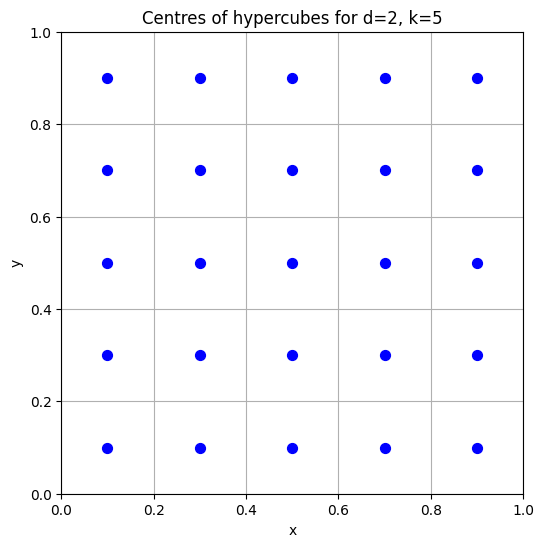
\includegraphics[width=0.4\linewidth]{points3.png}
            \caption{Principle of Haber's stratification}
            \label{fig:3}
        \end{figure}
    \end{frame}


 

    \begin{frame}{Haber vs. Quasi-Monte Carlo}
        \begin{itemize}
            \item<1->\textbf{Quasi-Monte Carlo (QMC):}
            \begin{itemize}
                \item Uses low-discrepancy sequences to fill \([0,1]^d\) more uniformly than i.i.d. random points.
                \item \textbf{Deterministic:} no randomness in sample generation.
                \item \textbf{RMSE Convergence:} The Root Mean Squared Error (RMSE) convergences at rate  \( \mathcal{O}(N^{-1} (\log N)^\frac{d}{2}) \) for functions of bounded variation.
    
            \end{itemize}
            
            \vspace{1em}
            
            \item<2->\textbf{Haber Estimators:}
            \begin{itemize}
                \item Use regular grid stratification \( \mathfrak{C}_k \subset [0,1]^d \) with \textbf{random perturbations} in each cell.
                \item \textbf{Unbiased Estimator:} Stratification minimizes bias by ensuring that each estimate is representative of the function's behavior over each subdomain.
                \item \textbf{Optimal RMSE Convergence:} RMSE converges at rate \( \mathcal{O}(N^{-1/2 - r/d}) \).
                \item \textbf{Minimization of the Variance:} subdomain are chosen to be as homogeneous as possible, thereby reducing the fluctuations of the function \( f(u) \) within each subdomain.
            \end{itemize}
        \end{itemize}
    \end{frame}

    \begin{frame}{Haber's estimator of order 1}
        \begin{itemize}
            \item<1-> Haber's estimator of order 1 is defined by
            $$\hat{I}_{1,k}(f) := \frac{1}{k^d} \sum_{c \in \mathfrak{C}_k} f(c + U_c), \quad U_c \sim \mathcal{U}\left(\left[-\frac{1}{2k}, \frac{1}{2k}\right]^d\right)$$
            \item<2-> Instead of randomly dropping samples everywhere, this method \textbf{ensures a uniform spatial coverage} by stratifying the domain into small subcubes.
        
            \item<3-> The perturbation $U_c$ inside each hypercube introduces \textbf{randomness}, allowing us to sample the function $f$ without relying solely on the midpoints.
        \end{itemize}
    \end{frame}

    \begin{frame}{Haber's estimator of order 1}
        \begin{figure}
            \centering
            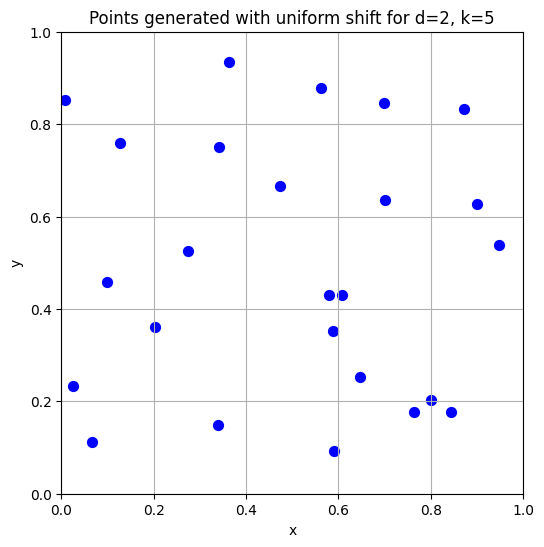
\includegraphics[width=0.4\linewidth]{points4.png}
            \caption{Stratification of Haber's estimator of order 1}
            \label{fig:4}
        \end{figure}
    \end{frame}

    \begin{frame}{Haber's estimator of order 2}
        \begin{itemize}
            \item<1-> Let
            $$g_c(u) := \frac{f(c + u) + f(c - u)}{2}$$
    
            Haber's estimator of order 2 is defined by 
            $$\hat{I}_{2,k}(f) := \frac{1}{k^d} \sum_{c \in \mathfrak{C}_k} g_c(U_c), \quad U_c \sim \mathcal{U}\left(\left[-\frac{1}{2k}, \frac{1}{2k}\right]^d\right)$$
    
            \item<2-> This estimator improves upon the first order by introducing a second level of perturbation within each subcube. This helps \textbf{increase the randomness} of the sampling process.
    
            \item<3-> The second perturbation introduces additional variability in the sampling points, making the estimator more robust and \textbf{reducing bias}.
    
        \end{itemize}
    \end{frame}

    \begin{frame}{Haber's estimator of order 2}
        \begin{figure}
            \centering
            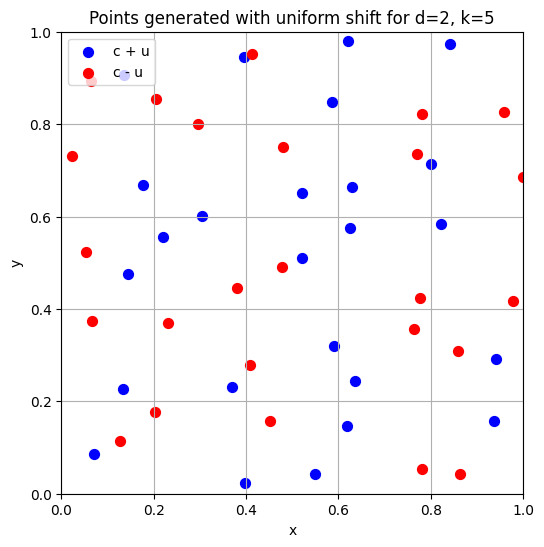
\includegraphics[width=0.4\linewidth]{points5.png}
            \caption{Stratification of Haber's estimator of order 2}
            \label{fig:5}
        \end{figure}
    \end{frame}




    \begin{frame}{Comparison of estimators}
        \begin{figure}
            \centering
            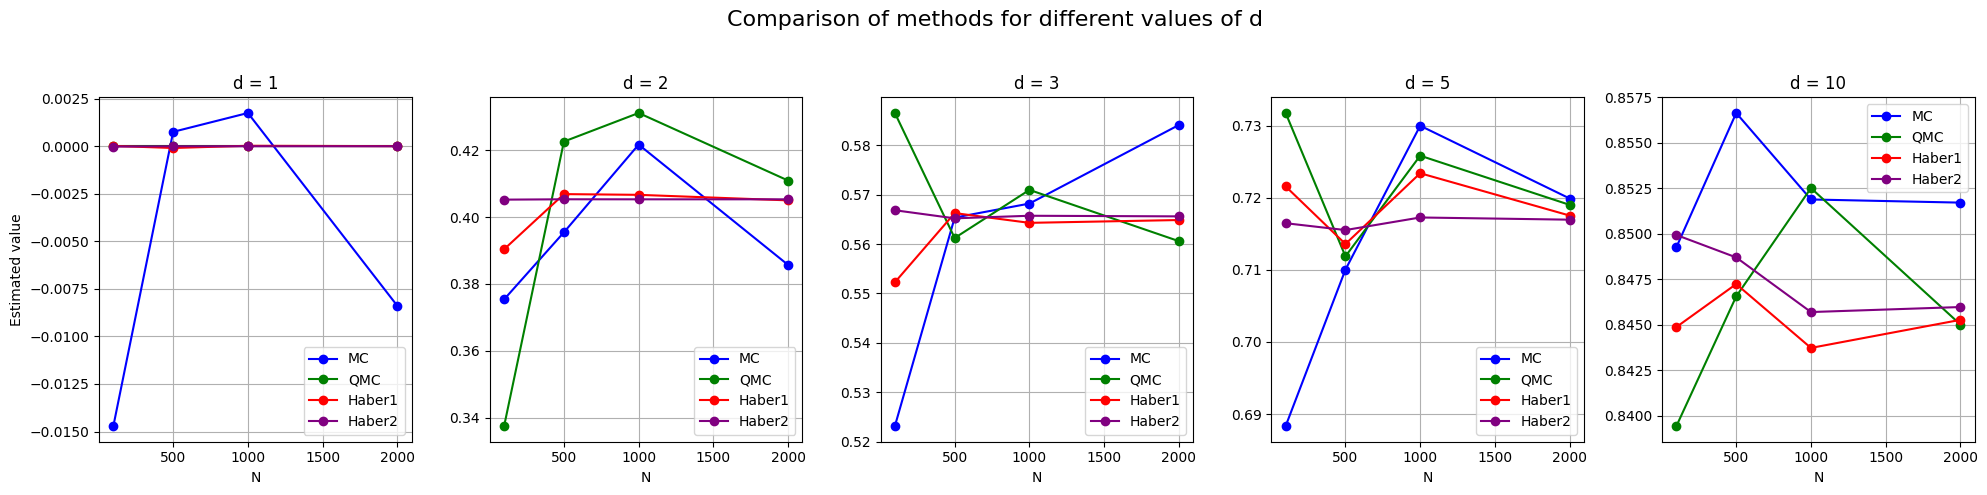
\includegraphics[width=1\linewidth]{graphs_haber.png}
            \caption{Comparison of estimators for different values of d and N}
            \label{fig:haber}
        \end{figure}

        \begin{itemize}
            \item To ensure fair comparison, we make the number of function evaluations comparable across methods by setting \( k = N^{1/d} \) in the Haber estimators.
        \end{itemize}
    \end{frame}
    %%%%% mettre à la fin et inclure un tableau où on compare les estimations et la variance pour différentes valeurs de k, d et N

    %%%%%%% limites du modèles
\begin{frame}{Limits of Haber Estimators}
    \begin{itemize}
        \item<1-> \textbf{Curse of dimensionality:} convergence rate \( \mathcal{O}(N^{-1/2 - r/d}) \) degrades with dimension \( d \); slow for high-dimensional problems.
        
        
        \item<2-> \textbf{Regularity assumptions:} optimal rates assume \( f \in \mathcal{C}^r([0,1]^d) \); not suitable for discontinuous or highly oscillatory functions.

        \item<3-> \textbf{No adaptive refinement:} fixed stratification cannot focus sampling effort on regions where \( f \) varies more.


    \end{itemize}
\end{frame}

    \section{Implementation of importance sampling methods}

    \begin{frame}{How does Importance Sampling work ?}
        \begin{itemize}
            \item<1-> We want to approximate the following integral:
            %
            \[I = \int_{[0,1]^d} f(x) \, dx\]

            \item<2-> We rewrite the integral as:
            %
            \[I = \int_{[0,1]^d} f(x) \, dx = \int_{[0,1]^d} \frac{f(x)}{g(x)} g(x) \, dx = \mathbb{E}_{X \sim g} \left[ \frac{f(X)}{g(X)} \cdot \bdOne_{X \in [0,1]^d} \right]\]
            %
            for any probability density function $g : \mathbb{R}^d \to \mathbb R$ satisfying $[0, 1]^d \subseteq \text{Supp}(g)$.\only<2->{\footnote{This assumption avoids division by zero.}} Such a density is called a \textbf{proposal density}.

            \item<3-> Thus, instead of approximating $\mathbb{E}[f(U)]$ where $U \sim \mathcal{U}([0, 1]^d)$, we now seek to approximate $\mathbb{E}\left[\frac{f(X)}{g(X)} \cdot \bdOne_{X \in [0,1]^d}\right]$ where the random vector $X$ is sampled from an appropriately chosen density $g$.
        \end{itemize}
    \end{frame}


    \begin{frame}
        \frametitle{How does Importance Sampling work ?}
        \begin{itemize}
            \item<1->We then draw \( x_1, x_2, \dots, x_N \overset{\text{i.i.d.}}{\sim} g \) and estimate:
        
            \[
            \hat{I} = \frac{1}{N} \sum_{i=1}^N \frac{f(x_i)}{g(x_i)} \cdot \bdOne_{x_i \in [0,1]^d}
            \]
    
            \vspace{1em}
             \item<2->The weight of each sample \( x_i \) is:
            \[
            w_i = \frac{f(x_i)}{g(x_i)} \quad \text{(only if \( x_i \in [0,1]^d \))}
            \]
        \end{itemize}
    \end{frame}




    

    \begin{frame}{Approximation of the integral using importance sampling}
    \begin{itemize}
            \item<1-> Assume that the input vector \( u = (u_1, \dots, u_d) \) consists of independent components, each uniformly distributed over \([0,1]\):
        \[
        u_i \sim \mathcal{U}([0, 1]), \quad \text{for } i = 1, \dots, d
        \]
        
        \bigskip
        \item<2->Then, for \( i = 1, \dots, d \), we have:
        \[
        \mathbb{E}[u_i] = \frac{1}{2}, \quad \mathrm{Var}(u_i) = \frac{1}{12}
        \]
        
        \item<3->By the Central Limit Theorem:
        \[
        \sqrt{d} \left( \bar{u}_d - \frac{1}{2} \right) \xrightarrow[d \to \infty]{\mathcal{L}} \mathcal{N}\left(0, \frac{1}{12}\right)
        \quad \text{with } \bar{u}_d = \frac{1}{d} \sum_{i=1}^d u_i
        \]

        \item<4->Consequently: for large values of $d$, the distribution of $\bar{u}_d$ is approximately $\mathcal{N}\left( \frac{1}{2}, \frac{1}{12d} \right)$.
        \end{itemize}
    \end{frame}
    
    \begin{frame}
    \frametitle{Histogram of simulations with normal approximation}

        Overlaying the histogram of simulations of \( \bar{u}_d \) from \( n = 10,000 \) simulations of \( u_1, \dots, u_d \), with the PDF of \( \mathcal{N}\left( \frac{1}{2}, \frac{1}{12d} \right) \), shows that this is a great approximation.
    
        \begin{center}
            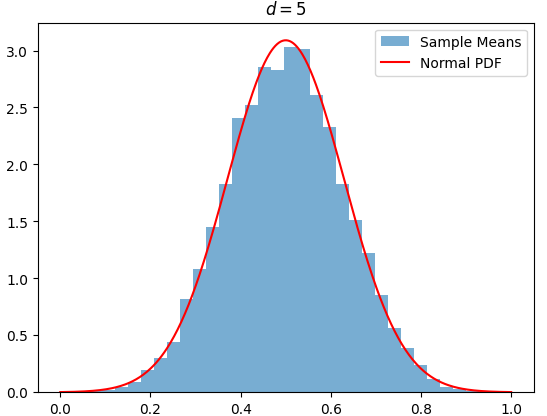
\includegraphics[width=0.32\textwidth]{mc1.PNG}
            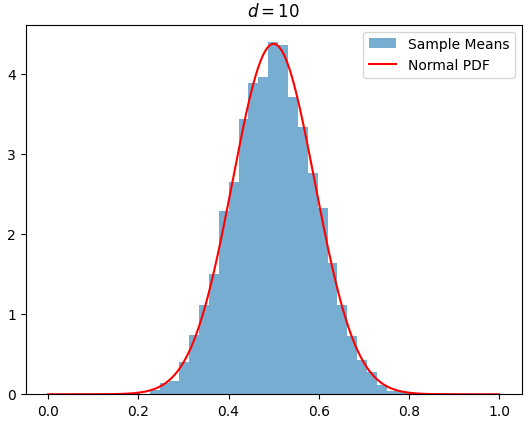
\includegraphics[width=0.32\textwidth]{mc2.PNG}
            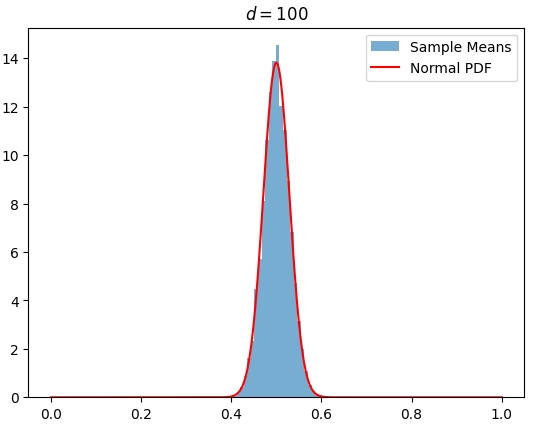
\includegraphics[width=0.32\textwidth]{mc3.PNG}
        \end{center}

    \end{frame}




    \begin{frame}
    \frametitle{Issue with the proposal density $g(x)$ in high dimensions}
        \begin{itemize}
            \item<1-> The previous observation encourages us to consider a density such that the marginal law of each component is $\mathcal{N}(\mu, \sigma^2)$, where $\mu = \frac{1}{2}$ and $\sigma^2 = \frac{1}{12d}$.

            For instance: choose $g$ $=$ the density of $\mathcal{N}_d\left(\left(\frac{1}{2}, \dots, \frac{1}{2}\right), \frac{1}{12d} I_d\right)$.

            \item<2-> \textbf{Issue:}
            \begin{itemize}
                \item<2-> When the dimension $d$ is large, the proposal distribution $g(x)$ becomes extremely concentrated around its mean.
                
                \item<3-> As a result, the density values $g(x)$ become very large in a small region.
                    
                \item<4-> This leads to importance weights $w(x) = \frac{f(x)}{g(x)}$ that are extremely small, often close to zero, making the estimator numerically unstable or biased toward zero.
            \end{itemize}
        \end{itemize}
    \end{frame}






    \begin{frame}
        \frametitle{Why is $g(x_i)$ huge in high dimension? 1}
        
        \begin{itemize}
            \item<1->We are using a multivariate normal distribution:
                \begin{itemize}
                  \item centered at $\mu = 0.5$
                  \item variance $\sigma^2 = \frac{1}{12d}$
                \end{itemize}
        
            \item<2->So the density is:
            \[
            g(x) = \prod_{j=1}^d \text{NormalPDF}(x_j ; 0.5, \sigma)
            \]
            
            \item<3->Each \texttt{NormalPDF} looks like:
            \[
            \frac{1}{\sqrt{2\pi \sigma^2}} \cdot e^{-\frac{(x_j - 0.5)^2}{2\sigma^2}}
            \]
        \end{itemize}
    \end{frame}

    \begin{frame}
        \frametitle{Why is $g(x_i)$ huge in high dimension? 2}
    
        \vspace{-1em}
        
        \begin{itemize}
            \item<1->\[
        g(x) = \prod_{j=1}^d \text{NormalPDF}(x_j ; 0.5, \sigma)
        \Rightarrow g(x) \text{ becomes very large near } x = 0.5
        \]
        
        \item<2->The smaller $\sigma$ is:
          \begin{itemize}
            \item the sharper the peak of the density
            \item $g(x)$ becomes very large around 0.5
          \end{itemize}
        
        \bigskip
        
        \item<3->So in the core of the density:
        \[
        g(x) \approx 10^{40},\ 10^{60},\dots \quad \Rightarrow \quad \frac{1}{g(x)} \approx 10^{-40},\ 10^{-60}
        \]
        \end{itemize}
    
    \end{frame}

    \begin{frame}
        \frametitle{Consequence}
        
        \begin{itemize}
            \item<1-> Even if:
            \begin{itemize}
              \item $f(x) \approx 1$
              \item $x \in [0,1]^d$
            \end{itemize}
        
            The weight:
            \[
            w(x) = \frac{f(x)}{g(x)} \approx \frac{1}{g(x)} \ll 1
            \]
        
            \vspace{1em}
                \item<2->$\Rightarrow$ Infinitesimal weight $\Rightarrow$ estimator becomes numerically close to 0
            
            \vspace{1em}
        
            \item<3->Because \textbf{$f$ only depends on the mean of the input}, and we're drawing values from a distribution that accurately reflects how that mean behaves, we don’t need to adjust with weights — just averaging the function values gives a reliable estimate.
        \end{itemize}
    \end{frame}


    \begin{frame}
    \frametitle{Testing the algorithm for multiple dimensions}
        We test importance sampling for different values of \( d \), and visualize the distribution for \( d = 10,000 \) with weight fiex at 1.

        \begin{center}
            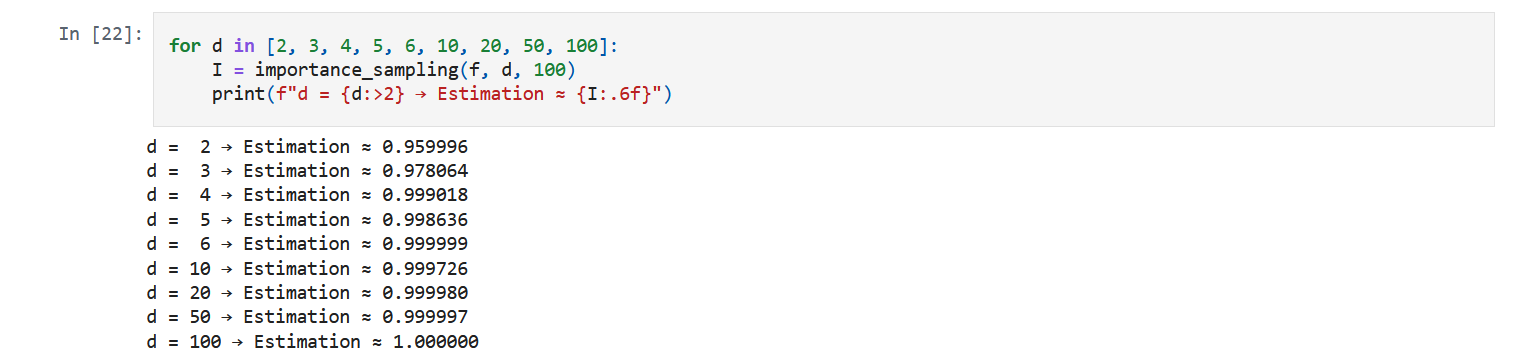
\includegraphics[width=1\textwidth]{projet_mc_output_d.png}
        \end{center}
    \end{frame}

    


    \begin{frame}
    \frametitle{Comparison of integration methods vs dimension}
        Let's visualize the convergence on a graph: $N = 1024$,
    
        \begin{center}
        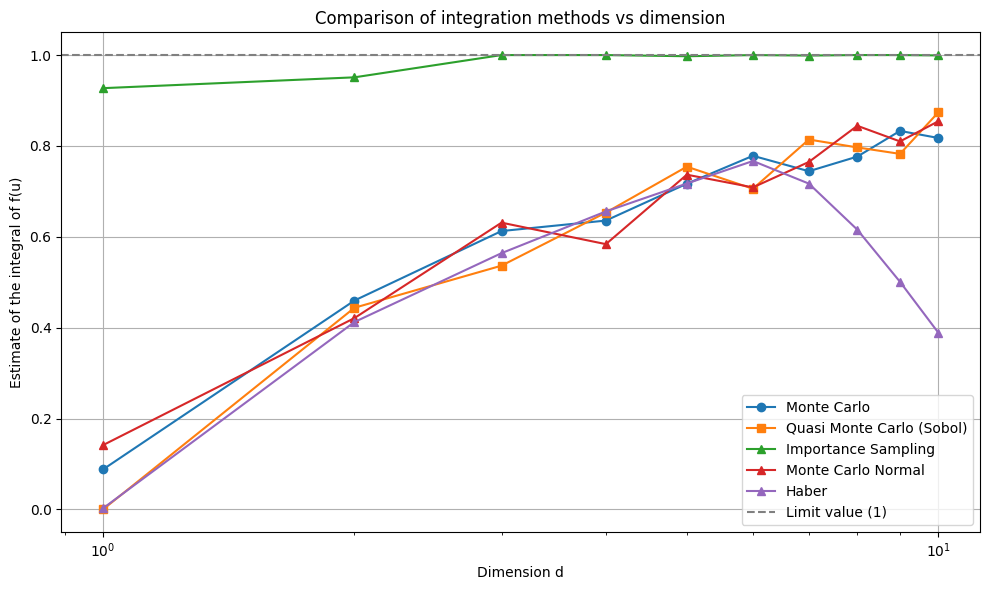
\includegraphics[width=0.75\textwidth]{output_compariaons mc.png}
        \end{center}
   

    \end{frame}



    
  
\end{document}